\section{Related Work}
%%%  Todo: Discussing "Practical SMT-based Type Error Localization"
Researchers have long realized that incomprehensible type errors result as a consequence of standard approaches to the type inference process. Many studied [Citation here] the approach of finding all locations that contribute to a type error. Haack and Wells~\cite{haack_type_2004} noted that ``\textit{Identifying only one node or subtree of the program as the error location makes it difficult for programmers to understand type errors. To choose the correct place to fix a type error, the programmer must find all the other program points that participate in the error.}''  Type error slicing~\cite{haack_type_2004} is a technique that finds locations that are complete and minimal for the type error. Internally labeled constraints and Minimal Unsatisfiable Set (MUS) manipulation are used to generate these slices. The language supported in Haack's work was a subset of Standard ML. The original Chameleon~\cite{stuckey_interactive_2003} used a similar technique but generate constraints in Constraint handling rules (CHR). As a result,  Chameleon supported advanced type-level features (type classes and functionally dependent types). The project also introduced the ability to query type information through a command line-style interface. Although Chameleon was firmly grounded in results from type theory, its designs were never evaluated with user studies.

One direction to approach type error debugging is by suggesting solutions to fix the type error. Sheng Chen's works \cite{chen_counter-factual_2014, chen_efficient_2020, chen_improving_2022} on counterfactual typing are able to suggest changes to make the ill-typed program type-check. While this is a promising ground, the work is not evaluated with human participants. \cite{lerner_searching_2007} studied an approach of repeatedly modifying the AST (abstract syntax tree) and querying the compiler/type checker to know whether the new program is well-typed. This approach allows the algorithm to suggest syntax changes that could fix the type error. Benefiting from not needing a type system implementation and being language agnostic, the underlying idea was implemented and evaluated in two different languages with ten university students. While suggesting syntax changes is very intuitive in practice, this approach has limitations for teaching and learning purposes, as it is not able to explain why the type errors occur and why fixes are suggested. The lack of explanation is due to the inquiry into the underlying type-check being a binary state. Deep type-level analysis (typing rules and language features) was not communicated to the inference algorithm.

Another related approach is through ECEM (Enhanced compiler error message). Through a series of mixed-method studies, Prather showed \cite{prather_novices_2017} that ECEM has a positive result in understanding compiler errors. Decafe \cite{becker_effective_2016} is a tool that can rephrase the Java compiler error messages into their enhanced version. In a study of over 200 CS1 students, Decaf was shown to reduce overall errors in their coding practices. Berik proposed a framework \cite{barik_how_2018} for constructing compiler error messages based on argumentation theory. In this proposal,  Berik argued that error messages following a simple argumentation layout or an extended argumentation layout are more human-friendly.  These works show the significance of improving the language in the compiler error messages. Most principles and suggestions are followed in \chameleon{} in constructing error statements. However, they were not targeting type errors alone but compiler errors (some even include run time errors) in general. The nuances of type errors, such as alternative typing, were not considered. 

% \begin{figure}[h]
%     \centering
%     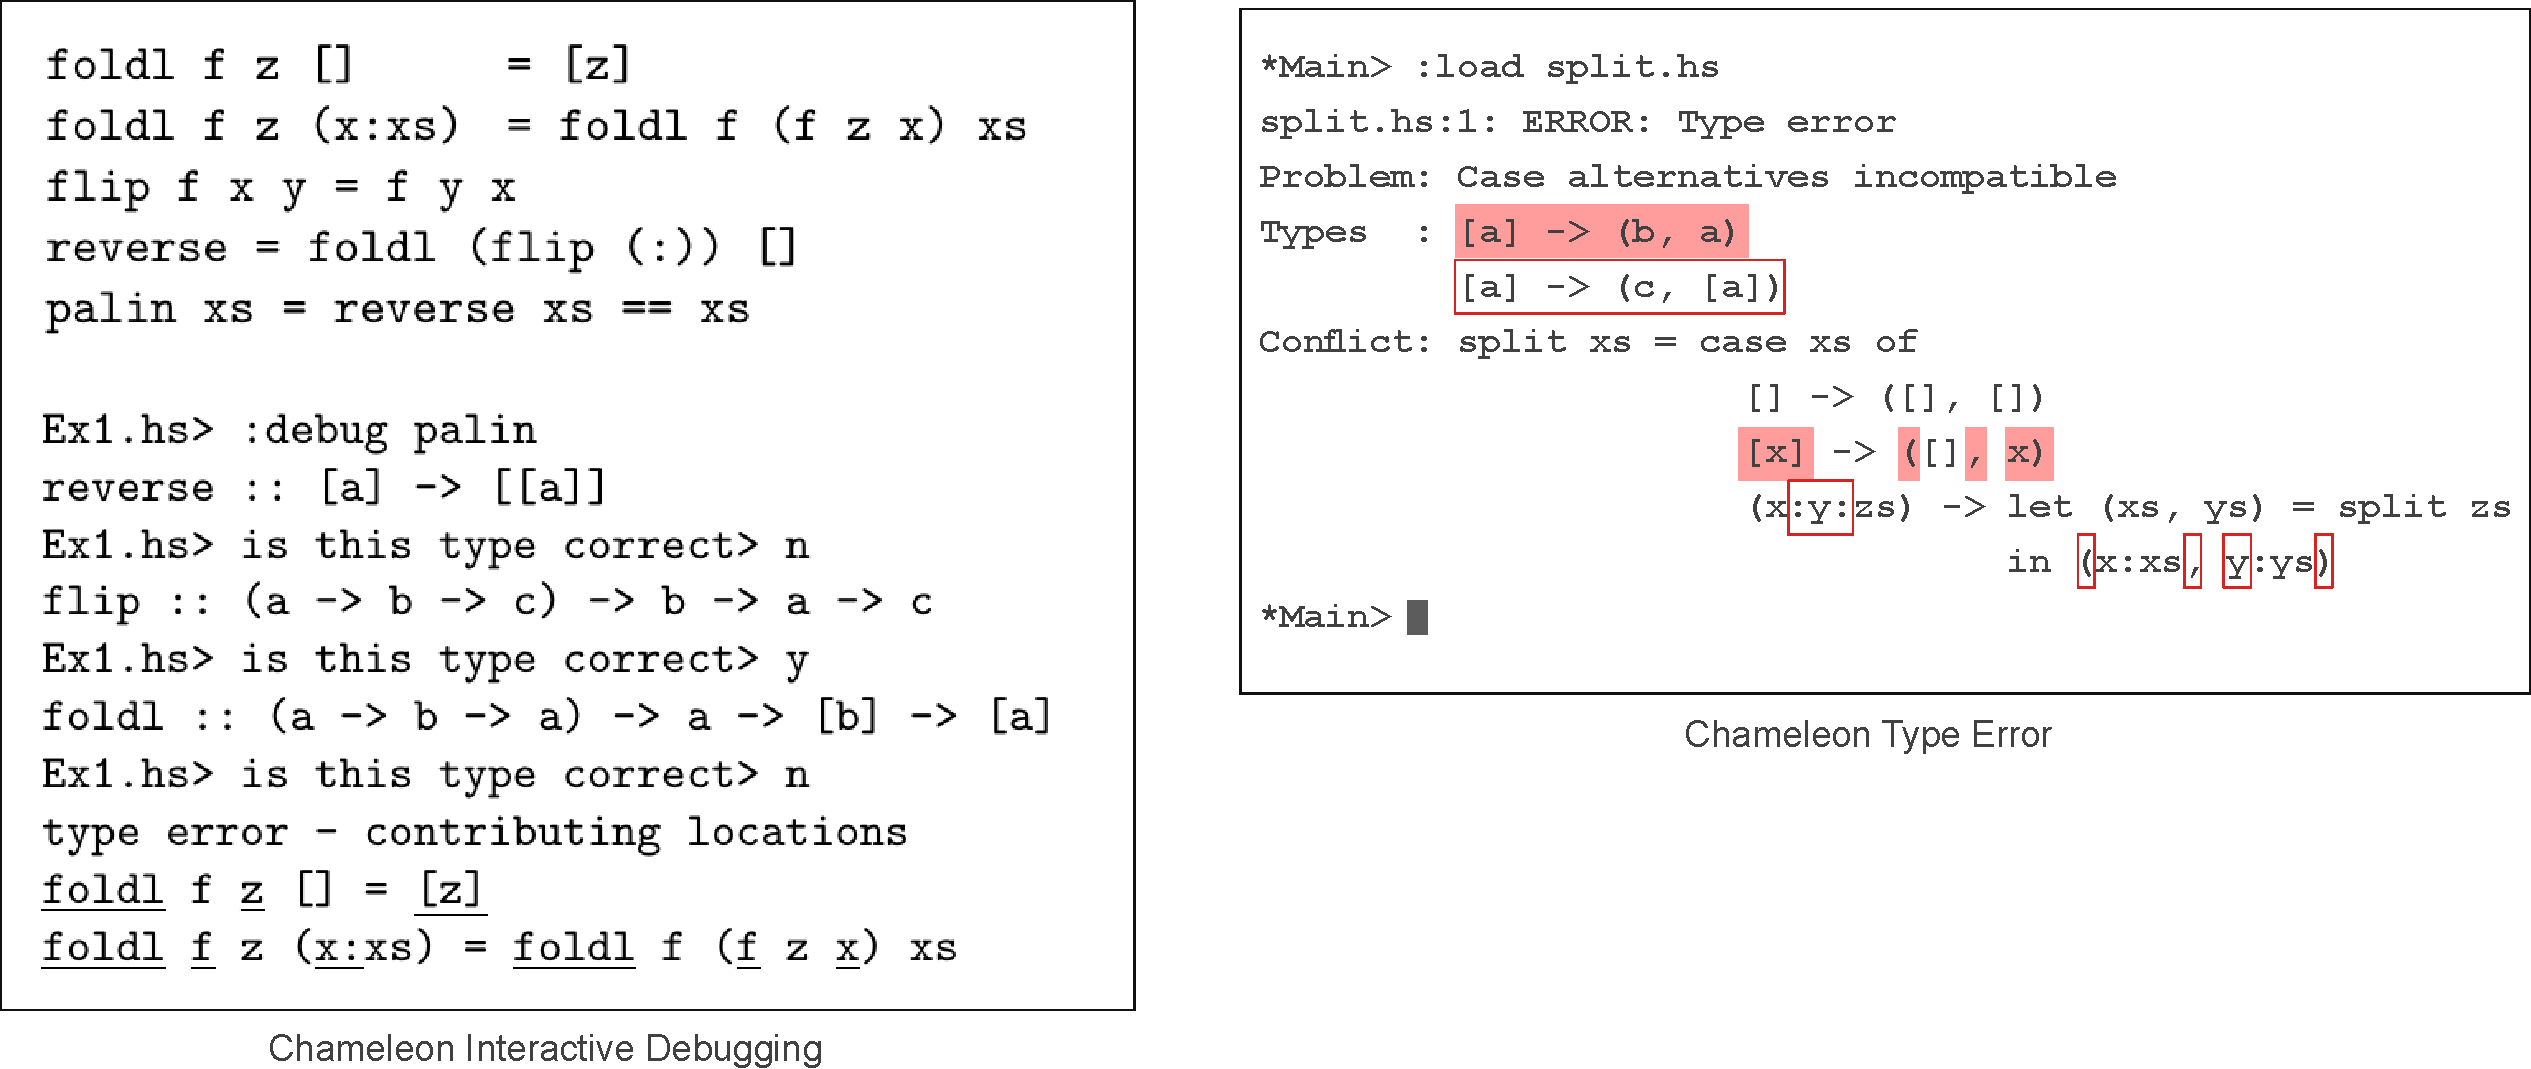
\includegraphics[width=\linewidth]{images/original-chameleon.pdf}
%     \caption{
% Originally, Chameleon was a command-line tool that can list all the potential causes of a type error and display the two branches in two forms of highlight (right), achieved with ASCII colors. In addition, it allows a few commands (debug and explain) in the debugging shell to help debug type errors (left).}
%     \label{fig:original-chameleon}
% \end{figure}


% The ChameleonIDE error reporting The error message of ChameleonIDE closely
% follows the argumentation structure outlined by Titus. Basic mode represent a
% simple structure argument, where the claim "The expression e can have two
% conflicting types" and the possible type 1 and two serves as grounds. When
% inspecting each possible types, the type judgements are treated as claim, and it
% is supported by the grounds: "Inferred from the orange/blue highlights on the
% left side". On the other hand, the similar type error message in GHC "Couldn't
% match expect type T1 with actual type T2" is "a ground masquerading as a clam",
% Barik commented. The balanced mode and advanced mode serve as a way to elaborate
% arguments from simple arguments into extended arguments.

% Another related topic is type-explanation~\cite{yang1999explaining, jun2002explaining}. Yang~\cite{jun2002explaining} showed an alternative type inference system capable of producing a human-like text explanation for why expressions are assigned certain types. A good explanation is drawn from surveying how human experts explain types. The resulting algorithm $\mathcal{H}$, generates a succinct explanation of the type inference steps to avoid using internal constructs (such as type variables). The explanation system has the advantage of acting like a human expert. However, when presented as text-based output, explanation systems have the potential to become verbose when types are complex or variable names are long. In \chameleon{}, we attempt to address this problem by showing one step of explanation at a time and referring to variables instead of spelling out the full name.


Debugging using a GUI Interactive Development Environment has been the standard practice for a long time. Compared to a command line-based interface, a graphic user interface provides programming tools that can show information hierarchy, provide immediate feedback to changes, and display complex visualizations. Hazel Tutor \cite{potter_hazel_2020} is an interactive type-driven environment for the OCaml language. It can automatically fill type holes by suggesting template expressions (strategies as called by the authors) through a popup window. It also provides a cursor-based type inspector that allows programmers to query the types of different parts of the program. Whyline~\cite{ko_finding_2009} is a Java debugging system that allows a user to ask questions like "why does variable X have value Y." It also allows users to interactively ask follow-up questions to gain further knowledge of the nature of an error.  These debugging tools are important motivations for developing \chameleon{}. However, they focus on different contexts of the debugging process. Java Whyline mainly tackles the problem of unintended run-time behavior, while Hazel Tutor specializes in interactive actions supporting type holes.


